%\addcontentsline{toc}{chapter}{Development Process}
\chapter{Final design}
This chapter will give an overview of the final design of the system reached by iteration 10. It will not go into detail for individual parts of the system as these were covered in the Iteration chapter but instead will offer a top level perspective of the system.

\section{Overall architecture}
The Laravel framework uses a Model-View-Controller design pattern\cite{mvc} to build applications. It works in the same way as a normal MVC application. Data is stored and manipulated within the models, controllers handle most of the interactions the user has with the system, and the views are the web pages presented to the users. Within Laravel, there is also a front controller, which is used to route incoming HTTP requests to the appropriate views and controllers\cite{Laravel-architechture}.

There are two sections of the system, the student end, and the lecturer end. The lecturer end is an admin panel that they can login to, to create and manage their quizzes. The student end consists of the portal for connecting to a session, and the session pages themselves that display the slides and questions for users to answer.

Students only have two bits of functionality available to  them, being able to join a quiz and then being able to answer questions. Lecturers however have more options on the site. On the admin backend they can create and edit new quizzes and questions, and add slides to the quizzes. They can also change their user details including their session key. The main operation they can perform is that they can run a quiz, this then takes them to the same view as the students, albeit with a small control panel for changing questions or slides, displaying the results of the quiz in real time and downloading the results. See \ref{fig:final-backend-use-case} and \ref{fig:final-frontend-use-case} for the two use case diagrams.

\begin{sidewaysfigure}
	\caption{Use case for backend of system}
	\centerline{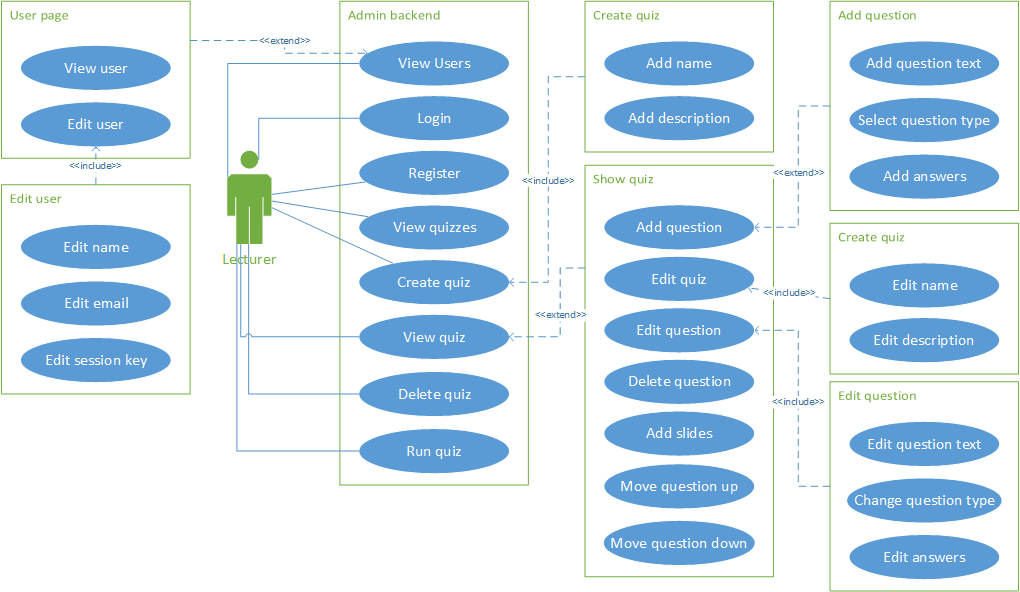
\includegraphics{Chapter3/final-backend-use-case}}
	\label{fig:final-backend-use-case}
\end{sidewaysfigure}

\begin{figure}
	\caption{Use case for frontend of system}
	\centerline{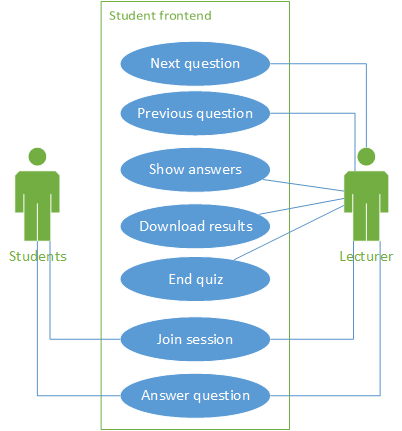
\includegraphics{Chapter3/final-frontend-use-case}}
	\label{fig:final-frontend-use-case}
\end{figure}

\newpage
Figure \ref{fig:overall-class-design} on the next page shows the overall class diagram, listing the models, controllers and groupings of views. The AuthController is a collection of controllers, however as they were generated by Laravel, they will not be shown in detail. The controllers all use various models, with the QuizController using them all. Future work might involve refactoring these controllers as some functionality could be separated into sub controllers.

The views shown in the image are also collections of views, as showing each and every view would take up too much room, however they all fall under those top levels.

\begin{sidewaysfigure}
	\caption{Class design for final system}
	\centerline{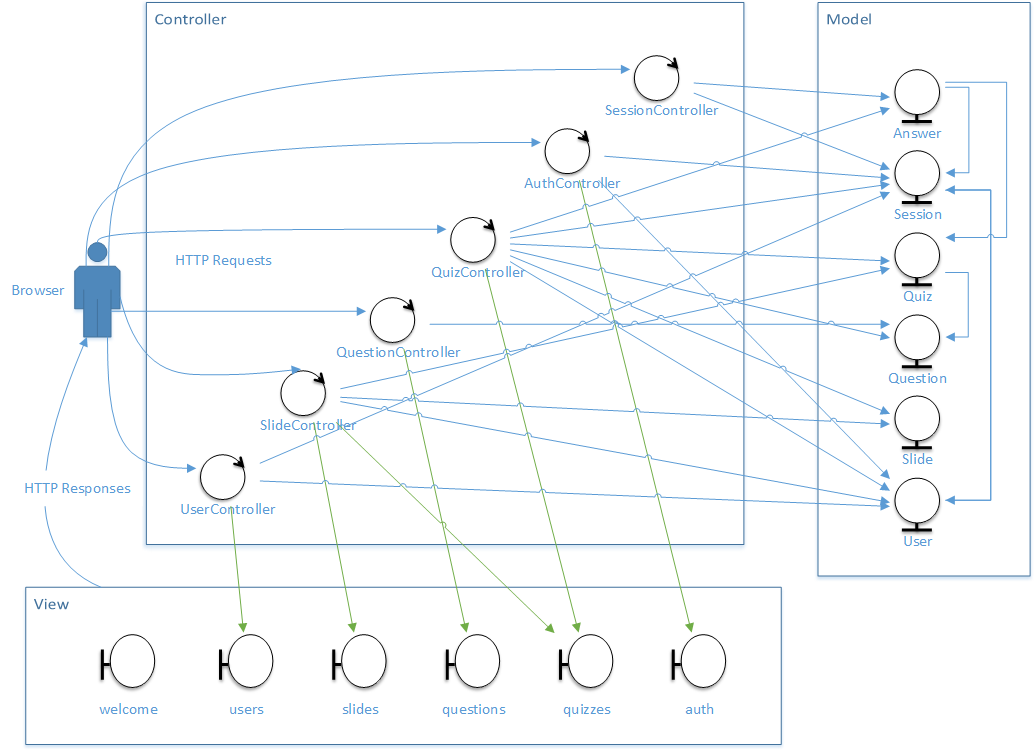
\includegraphics{Chapter3/overall-class-design}}
	\label{fig:overall-class-design}
\end{sidewaysfigure}

\newpage
\section{Database design}
Figure \ref{fig:er-diagram} shows the seven tables within the application. Two of these were generated by running a Laravel command to make the authentication part of the site, the users and password\_resets tables. These provide basic user authentication. the other five, answers, questions, quizzes, sessions and slides were made manually.

The quizzes table contains information about the quizzes themselves, and are associated with a user. The questions and slides tables both store information about their respective parts of a quiz, with each row within these tables associated with a quiz. Questions store information about the actual question including all the answers. Not present in the design  for the answers table above are the other eight fields for answers up to answer10. The slides table stores the file name of a slide image that has been converted from a pdf slide. Both of these tables store the positions of their items within a quiz.

The sessions table stores the information about the runnable session, each user has one associated session row. Within this row, the session\_key is stored, which is the key that students would use to connect to a session. Additionally it stores information about the session when it is running, specifying if it is running, and what position it is at. This position references the positions specified in the questions and slides tables, though there is no actual foreign key relationship between them. 

The final table, answers, stores all the responses from users to questions. It stores which question, the answer given and the user that submitted the answer. The user\_session is a cookie value rather than a user from the database.

\begin{sidewaysfigure}
	\caption{Entity relationship digram for final database}
	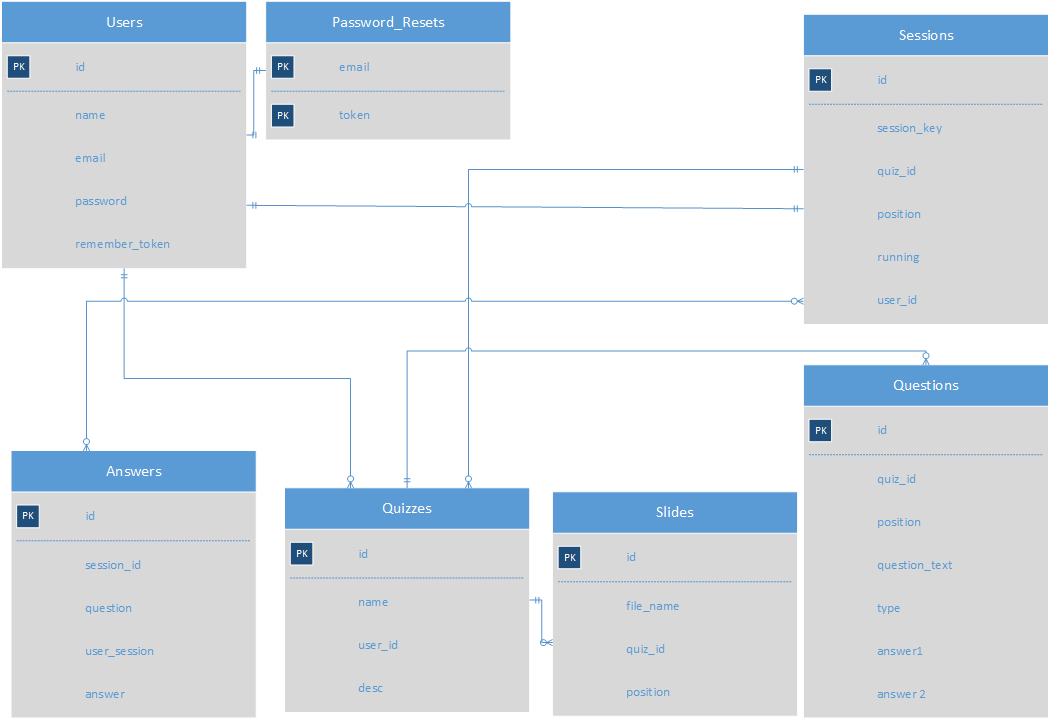
\includegraphics[width=\textwidth]{Chapter3/Final-ER-Image}
	\label{fig:er-diagram}
\end{sidewaysfigure}